\section{数据与实验思路}
\subsection{先区分采样现象与位置错误}
课程提供的轨迹数据\cite{teacher}包含11,386条记录，共1,173,410个观测点。每条记录由相互对应的时间序列和坐标序列组成，记录内共有1,162,024对相邻观测。文件中的记录键用于区分这些序列，并不提供用户身份或完整行程信息。

选择处理方法之前，需要先看清数据中出现了什么。全量检查得到表\ref{tab:data}中的四类现象。相邻坐标完全相同的情况较多；同时，也存在时间差为零但坐标不同，以及采样间隔超过30秒的情况。这些统计描述的是观测特征，不是已经标注好的噪声类别。

\begin{table}[htbp]\centering
\caption{原始轨迹的部分采样现象}\label{tab:data}
\small\renewcommand{\arraystretch}{1.28}
\begin{tabularx}{\linewidth}{@{}Yrr@{}}\toprule
相邻观测的特征 & 数量 & 占相邻观测对的比例\\\midrule
位置完全相同 & 575,278 & 49.51\%\\
时间差为零 & 42,185 & 3.63\%\\
同一时刻、不同位置 & 29,175 & 2.51\%\\
时间差超过30秒 & 8,272 & 0.71\%\\\bottomrule
\end{tabularx}
\vspace{3.5mm}
\begin{minipage}{\linewidth}\footnotesize\color{Muted}
统计单位为同一记录内的相邻观测对，比例分母均为1,162,024。不同现象可能重叠，数量不能相加作为异常点总数；30秒在此用于描述采样间隔，是否适合作为分段阈值将在后文比较。
\end{minipage}
\end{table}

\subsection{直接连线与直接删点各有什么风险}
若把所有相邻观测直接连接，较长的采样空档也会被画成一条连续线段，而空档期间的实际路径并未被记录。另一方面，相同坐标在不同时间出现，可能包含停留信息，不能仅因位置重复就直接删除。同一时刻出现不同位置时，相邻速度也无法由距离除以时间差得到；实验保留这种不可计算情况，而不是把速度填成零。

局部方向突变同样需要进一步检查：它可能来自位置异常，也可能是真实折返。分段、方向去噪与简化分别面对连接、局部形状和点数冗余问题，不能只凭轨迹看起来更平滑，就认定处理更准确。

\clearpage
\subsection{把空间位置与采样时间一起观察}
只看二维连线，相同位置的多次观测容易叠在一起。图\ref{fig:space-time}将记录352的170个观测点沿相对时间展开，并叠加后文最终方案的处理结果，便于同时观察采样先后、片段连接和保留点的位置。本例用于解释处理关系，整体效果仍由后续样本与全量结果判断。

\begin{figure}[htbp]\centering
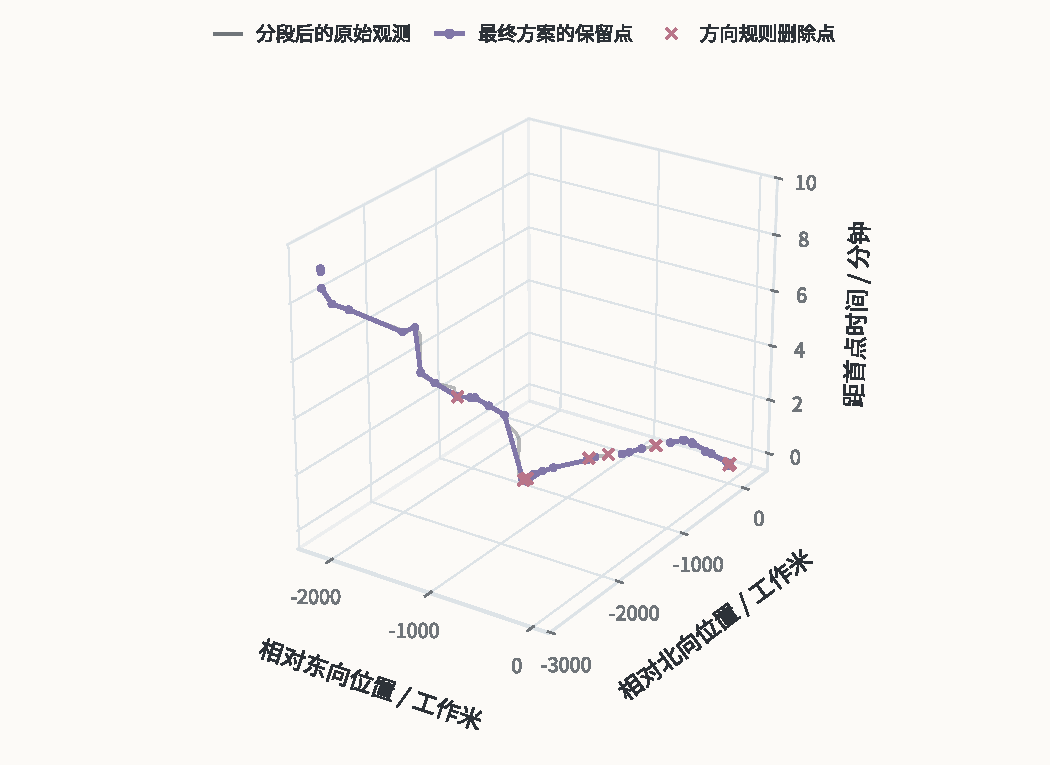
\includegraphics[width=.98\linewidth]{figures/G1A_space_time.pdf}
\caption{记录352的三维时空表示。灰线为分段后的原始观测，紫线连接最终方案保留的点，叉号标出方向规则删除点；各片段之间不连线。空间位置仅平移至首点，竖轴为相对时间而非海拔，也不参与平面距离计算。}\label{fig:space-time}
\end{figure}

数据文件未注明坐标参考系。实验使用固定椭球模型，将经纬度数值转换至同一局部平面，统一计算距离和方向。下文以“工作米”表示这一模型中的长度，用于方案间比较，不代表已经确认的真实定位精度；具体转换与核对方法放在方法说明及附录中。

\subsection{怎样从处理结果中选择方案}
仅看删除数量，容易奖励丢弃大量数据的方案；仅看最后一步的误差，又可能忽略前面已经删除的点。因此，实验先核对各步骤是否按定义执行，再使用同一原始参考比较覆盖、几何偏差和压缩效果。局部检查合格，是继续比较的前提，不是采用方案的充分理由。

后续先分别改变参数与处理顺序，保留各项独立结果；有依据的调整才进一步组合。LLM提出的设置也进入相同的处理和核验过程。结果满足比较条件时继续验证，出现退化则保留原方案；实现错误修正后重算，方法没有收益则如实记录。下一章先说明三种处理操作及其检查方式，再展开方案之间的比较。

